\documentclass[a4paper]{report}
\usepackage[utf8]{inputenc}
\usepackage[T1]{fontenc}
\usepackage{textcomp}

\usepackage{url}

% \usepackage{hyperref}
% \hypersetup{
%     colorlinks,
%     linkcolor={black},
%     citecolor={black},
%     urlcolor={blue!80!black}
% }

\usepackage{graphicx}
\usepackage{float}
\usepackage[usenames,dvipsnames]{xcolor}

% \usepackage{cmbright}

\usepackage{amsmath, amsfonts, mathtools, amsthm, amssymb}
\usepackage{mathrsfs}
\usepackage{cancel}

\newcommand\N{\ensuremath{\mathbb{N}}}
\newcommand\R{\ensuremath{\mathbb{R}}}
\newcommand\F{\ensuremath{\mathscr{F}}}
\newcommand\Z{\ensuremath{\mathbb{Z}}}
\renewcommand\O{\ensuremath{\emptyset}}
\newcommand\Q{\ensuremath{\mathbb{Q}}}
\newcommand\C{\ensuremath{\mathbb{C}}}
\let\implies\Rightarrow
\let\impliedby\Leftarrow
\let\iff\Leftrightarrow
\let\epsilon\varepsilon

% horizontal rule
\newcommand\hr{
    \noindent\rule[0.5ex]{\linewidth}{0.5pt}
}

\usepackage{tikz}
\usepackage{tikz-cd}

% theorems
\usepackage{thmtools}
\usepackage[framemethod=TikZ]{mdframed}
\mdfsetup{skipabove=1em,skipbelow=0em, innertopmargin=5pt, innerbottommargin=6pt}

\theoremstyle{definition}

\makeatletter

\declaretheoremstyle[headfont=\bfseries\sffamily, bodyfont=\normalfont, mdframed={ nobreak } ]{thmgreenbox}
\declaretheoremstyle[headfont=\bfseries\sffamily, bodyfont=\normalfont, mdframed={ nobreak } ]{thmredbox}
\declaretheoremstyle[headfont=\bfseries\sffamily, bodyfont=\normalfont]{thmbluebox}
\declaretheoremstyle[headfont=\bfseries\sffamily, bodyfont=\normalfont]{thmblueline}
\declaretheoremstyle[headfont=\bfseries\sffamily, bodyfont=\normalfont, numbered=no, mdframed={ rightline=false, topline=false, bottomline=false, }, qed=\qedsymbol ]{thmproofbox}
\declaretheoremstyle[headfont=\bfseries\sffamily, bodyfont=\normalfont, numbered=no, mdframed={ nobreak, rightline=false, topline=false, bottomline=false } ]{thmexplanationbox}


\declaretheorem[numberwithin=chapter, style=thmgreenbox, name=Definition]{definition}
\declaretheorem[sibling=definition, style=thmredbox, name=Corollary]{corollary}
\declaretheorem[sibling=definition, style=thmredbox, name=Proposition]{prop}
\declaretheorem[sibling=definition, style=thmredbox, name=Theorem]{theorem}
\declaretheorem[sibling=definition, style=thmredbox, name=Lemma]{lemma}



\declaretheorem[numbered=no, style=thmexplanationbox, name=Proof]{explanation}
\declaretheorem[numbered=no, style=thmproofbox, name=Proof]{replacementproof}
\declaretheorem[style=thmbluebox,  numbered=no, name=Exercise]{ex}
\declaretheorem[style=thmbluebox,  numbered=no, name=Example]{eg}
\declaretheorem[style=thmblueline, numbered=no, name=Remark]{remark}
\declaretheorem[style=thmblueline, numbered=no, name=Note]{note}

\renewenvironment{proof}[1][\proofname]{\begin{replacementproof}}{\end{replacementproof}}

\AtEndEnvironment{eg}{\null\hfill$\diamond$}%

\newtheorem*{uovt}{UOVT}
\newtheorem*{notation}{Notation}
\newtheorem*{previouslyseen}{As previously seen}
\newtheorem*{problem}{Problem}
\newtheorem*{observe}{Observe}
\newtheorem*{property}{Property}
\newtheorem*{intuition}{Intuition}


\usepackage{etoolbox}
\AtEndEnvironment{vb}{\null\hfill$\diamond$}%
\AtEndEnvironment{intermezzo}{\null\hfill$\diamond$}%




% http://tex.stackexchange.com/questions/22119/how-can-i-change-the-spacing-before-theorems-with-amsthm
% \def\thm@space@setup{%
%   \thm@preskip=\parskip \thm@postskip=0pt
% }

\usepackage{xifthen}

\def\testdateparts#1{\dateparts#1\relax}
\def\dateparts#1 #2 #3 #4 #5\relax{
    \marginpar{\small\textsf{\mbox{#1 #2 #3 #5}}}
}

\def\@lesson{}%
\newcommand{\lesson}[3]{
    \ifthenelse{\isempty{#3}}{%
        \def\@lesson{Lecture #1}%
    }{%
        \def\@lesson{Lecture #1: #3}%
    }%
    \subsection*{\@lesson}
    \testdateparts{#2}
}

% fancy headers
\usepackage{fancyhdr}
\pagestyle{fancy}

% \fancyhead[LE,RO]{Gilles Castel}
\fancyhead[RO,LE]{\@lesson}
\fancyhead[RE,LO]{}
\fancyfoot[LE,RO]{\thepage}
\fancyfoot[C]{\leftmark}
\renewcommand{\headrulewidth}{0pt}

\makeatother

% figure support (https://castel.dev/post/lecture-notes-2)
\usepackage{import}
\usepackage{xifthen}
\pdfminorversion=7
\usepackage{pdfpages}
\usepackage{transparent}
\newcommand{\incfig}[1]{%
    \def\svgwidth{\columnwidth}
    \import{./figures/}{#1.pdf_tex}
}

% %http://tex.stackexchange.com/questions/76273/multiple-pdfs-with-page-group-included-in-a-single-page-warning
\pdfsuppresswarningpagegroup=1

\author{Aamod Varma}
\setlength{\parindent}{0pt}


\title{MATH3012}
\author{Aamod Varma}
\usepackage{graphicx}
\graphicspath{ {./}}
\begin{document}
\maketitle


\section*{Keller and Trotter}

\section*{5.9}

\subsection*{Problem 36}
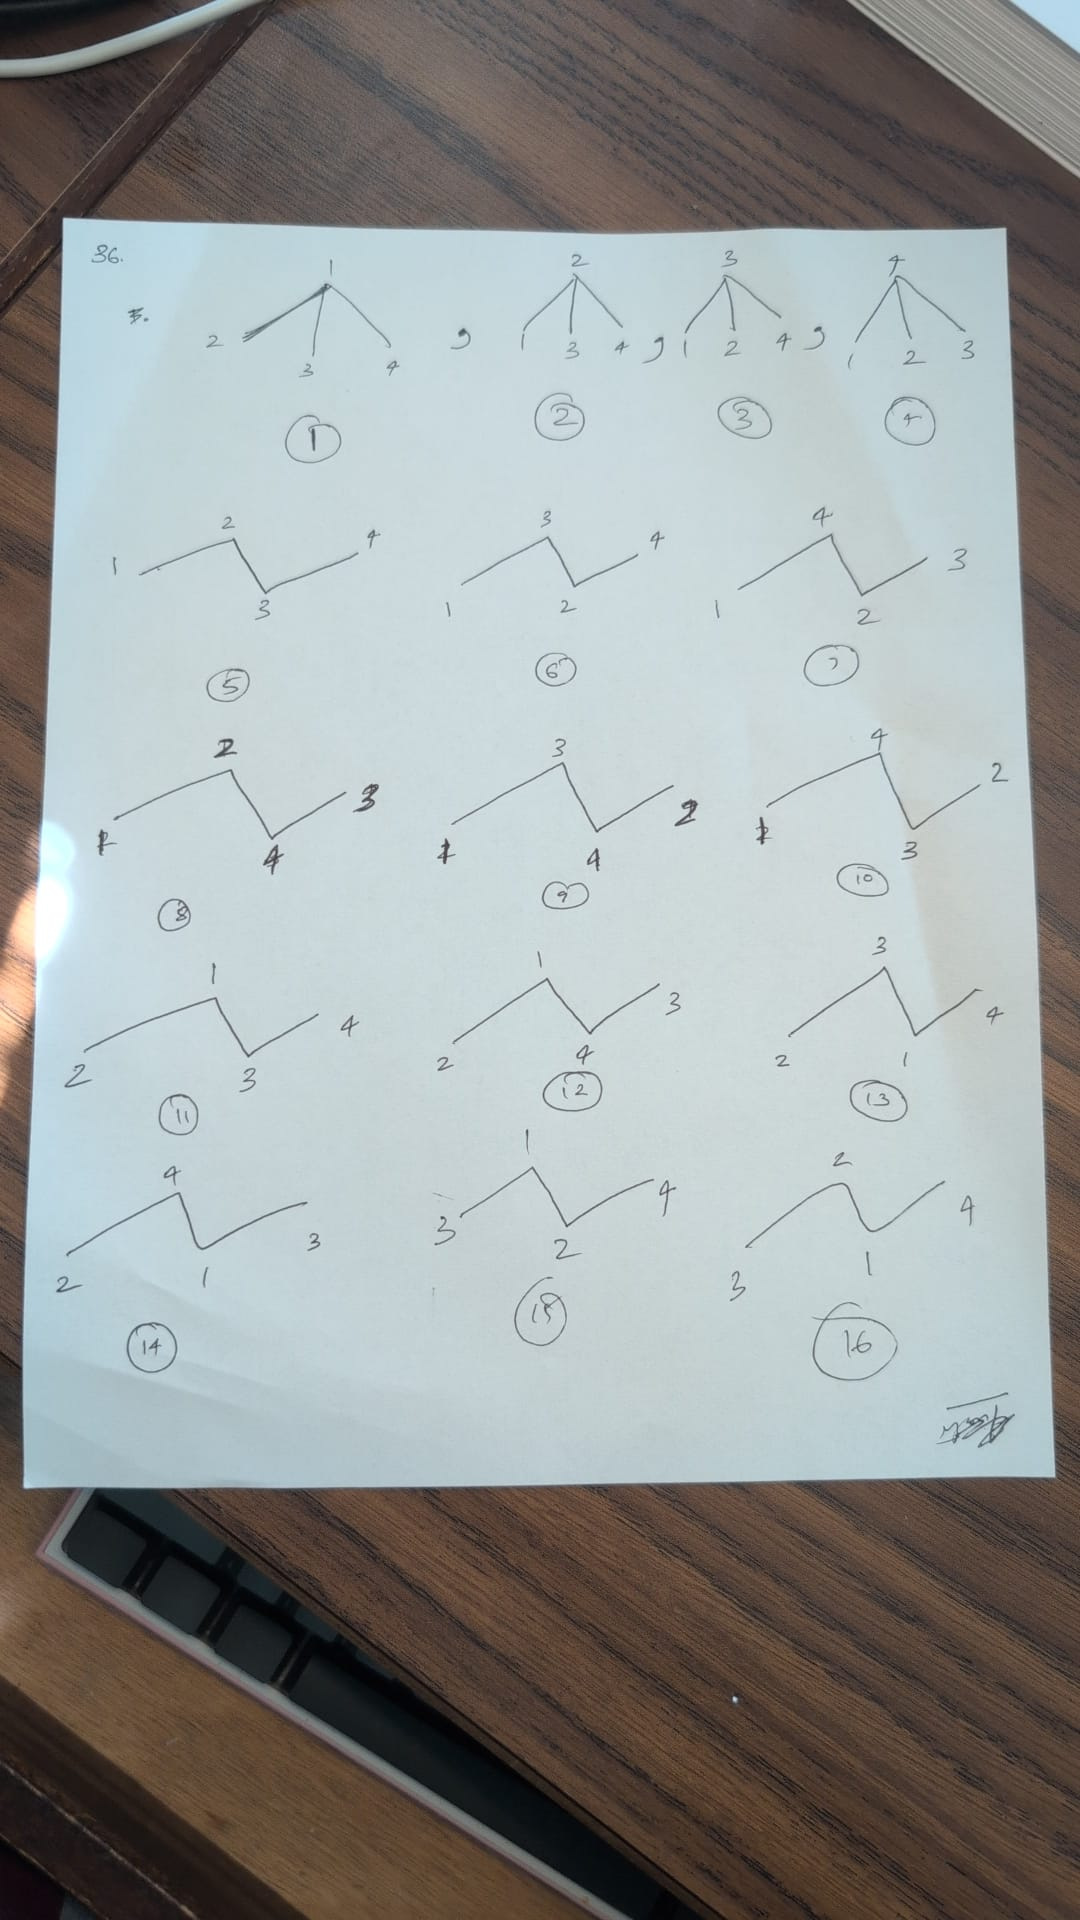
\includegraphics[scale=.25]{36}
\subsection*{Problem 37}
The prufer code for this tree would be $1,4,6,9,4,9,1,4$

\subsection*{Problem 40}
\begin{align*}
    &9,6,1,1,3,4,7,3 \qquad &\{1,2,3,4,5,6,7,8,9,10\} \\
    &6,1,1,3,4,7,3 \qquad &\{1,3,4,5,6,7,8,9,10\} \\
    &1,1,3,4,7,3 \qquad &\{1,3,4,6,7,8,9,10\} \\
    &1,3,4,7,3 \qquad &\{1,3,4,7,8,9,10\} \\
    &3,4,7,3 \qquad &\{1,3,4,7,9,10\} \\
    &4,7,3 \qquad &\{3,4,7,9,10\} \\
    &7,3 \qquad &\{3,4,7,10\} \\
    &3 \qquad &\{3,7,10\} \\
    &\text{empty string} \qquad &\{3,10\} \\
\end{align*}

This gives us the following graph,

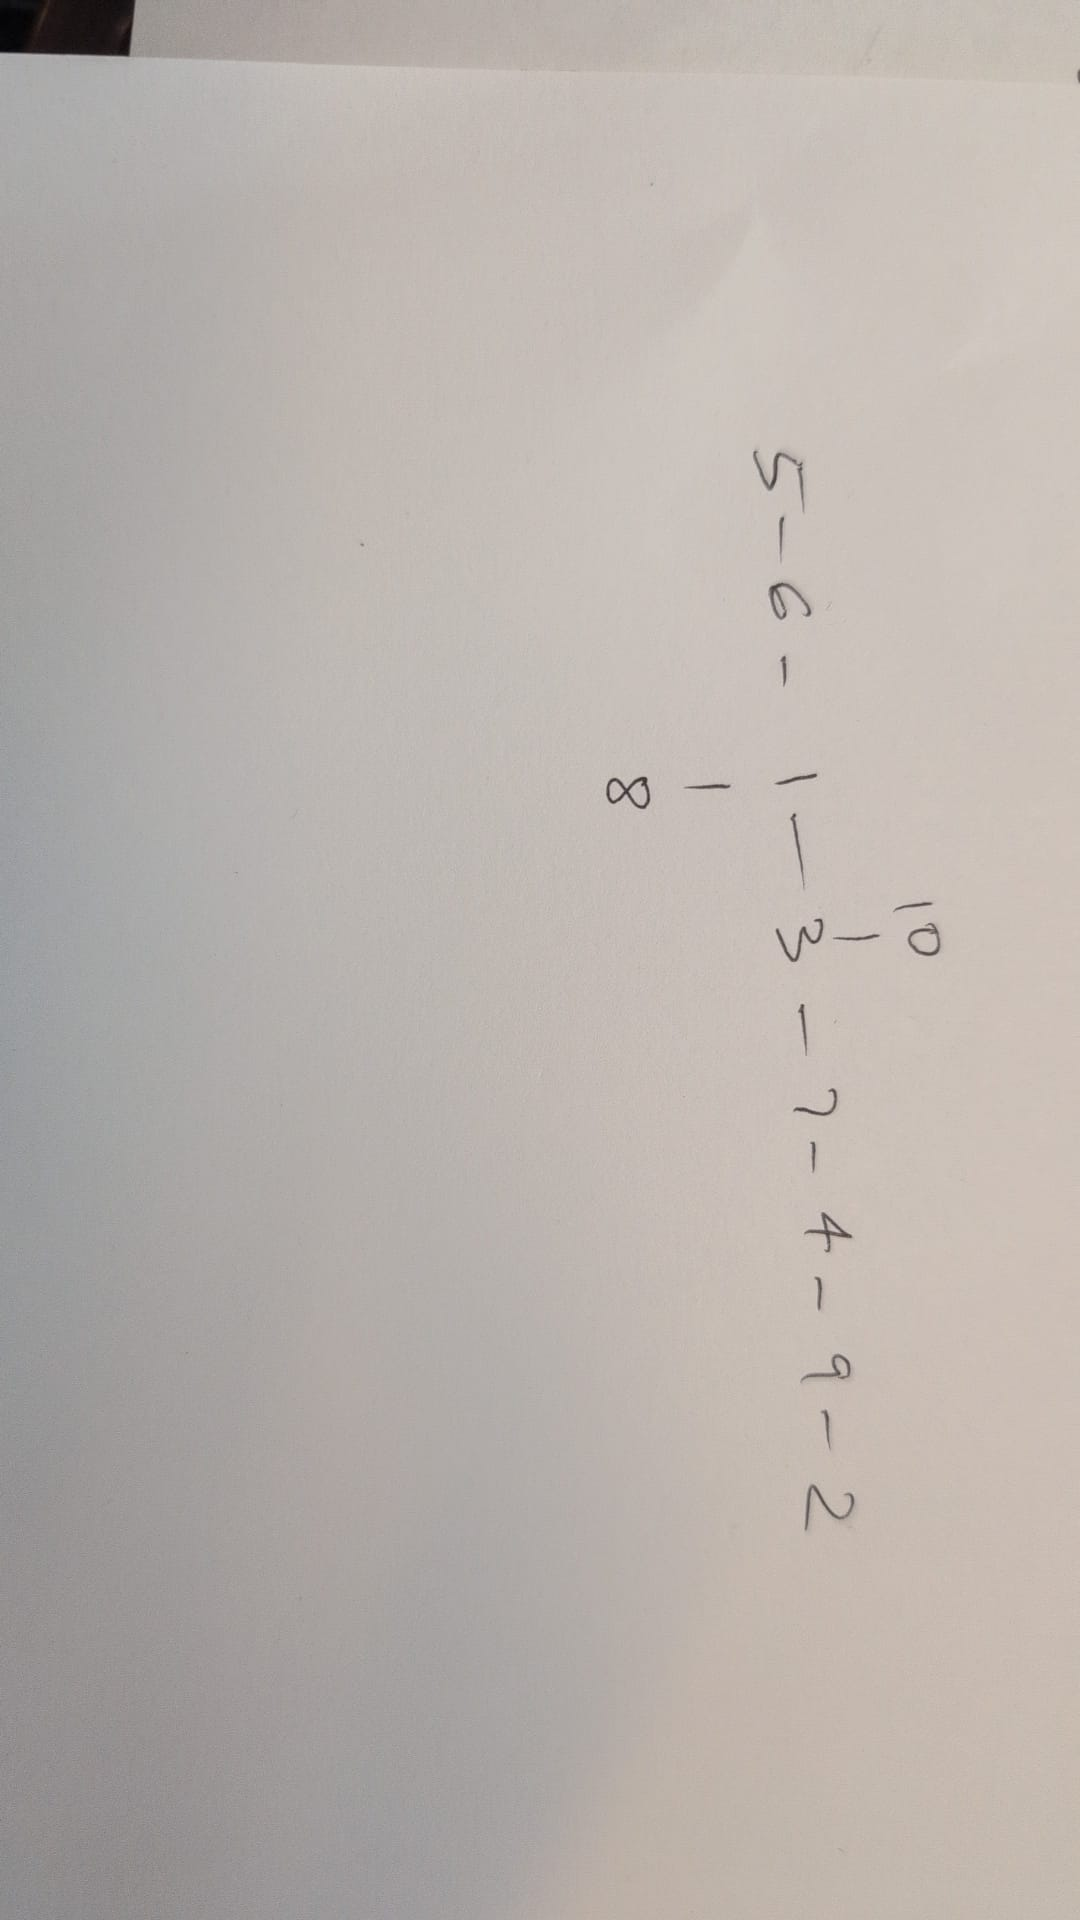
\includegraphics[angle=90,scale=.20]{40}


\section*{6.10}


\subsection*{Problem 1}
To count the symmetric relations we can first check the way we can choose 2 elements from the list $\{a,b,c,d,e,f\}$ including repetitions. This is equivalent to finding num of solutions to, 
$$ x_1 + \dots + x_6 = 2  \qquad \text{where $x_i \ge 0$} $$ 

This has the num of solutions as $7 \choose 2$ which is 21.

Now for each element in this 21 we can add it's reverse to  $R$ to create a symmetric relation so either they can exist in R or not which means we have 2 options for each of the 21 pairs of numbers which gives us a total of, 
$$ 2^{21}  \text{ relations that are symmetric}$$ 

Now out of the $21$ we have $6$ elements that are self pairs i.e. $(a,a),\dots,(f,f)$. So without repetition we have $21 - 6 = 15$ pairs. Now to get a reflexive relation we need for all $x \in X, xRx$. So  $R$ must include these pairs. For the remaining 15 they can either be in $R$. So fixing  these 6  we will have a total of, 
$$ 2^{15} \text{ relations that are reflexive and symmetric}$$ 
\subsection*{Problem 2}
We have the relation, 
$$ aRb \: (a,b \in \Z) \iff  a \equiv b \pmod{m}$$ 

1. Reflexive

We need to show $\forall x \in Z, xRx$  or $x \equiv x \pmod{m}$. We have, 
\begin{align*}
    x &\equiv x \pmod{m}\\
    x - x &= km \qquad \text{for $k \in \Z$}\\
    0 &= km \qquad \text{$k \in \Z$}
\end{align*}

So for $k = 0$ this is true. Hence we have $x \equiv x \pmod{m}$ for any  $m \ge 2$.

2. Symmetric

We need to show that  for $x,y \in \Z,  xRy \implies yRx$. Or that,  
$$ x \equiv y \pmod m \implies y \equiv x \pmod m $$ 

We have the following, 
\begin{align*}
    x&Ry\\
    x &\equiv y \pmod m\\
    x - y &= km \qquad &\text{for $k \in \Z$}\\
    y - x &= (-k)m \qquad &\text{for $k \in \Z$}\\
    y - x &= (k')m \qquad &\text{as $k' = -k \implies k' \in \Z$}\\
    y &\equiv x  \pmod m \qquad \\
    y&Rx
\end{align*}

hence we showed that for $x,y \in R$  that $xRy \implies yRx$ which means it is symmetric.


3. Transitive

We need to show that  $xRy, yRz \implies xRz$. First we have, 
\begin{align*}
    x&Ry \\
    x &\equiv y \pmod m\\
    x - y &= km \qquad \text{ for $k \in \Z$}
\end{align*}

Similar we have, 

\begin{align*}
    y&Rz \\
    y &\equiv z \pmod m\\
    y - z &= qm \qquad \text{ for $q \in \Z$}
\end{align*}


Now adding the final from both we have, 
\begin{align*}
    x - y + y - z &= km + qm\\
    x - z &= (k + q)m\\
    x - z &= rm \qquad \text{$k,q \in \Z \implies r = k + q \in \Z$}\\
    x&Rz
\end{align*}

Hence we have shown that $xRy, yRz \implies xRz$ which completes the proof for transitivity.



So we have shown that $R$ is reflexive, symmetric and transitive which implies that it is an equivalence relation.

\subsection*{Problem 3}
First we see that $P$ is not reflexive as $(5,5) \not \in P$ so this itself makes it not a partial order. 

We see that it is not symmetric which is what we want. And lastly we see that it is transitive as for any $(x,y), (y,z) \in R$ we have  $(x,z) \in P$.

So if we add  $(5,5)$ to  $P$ we have a partial order on the set $X$
\subsection*{Problem 4}

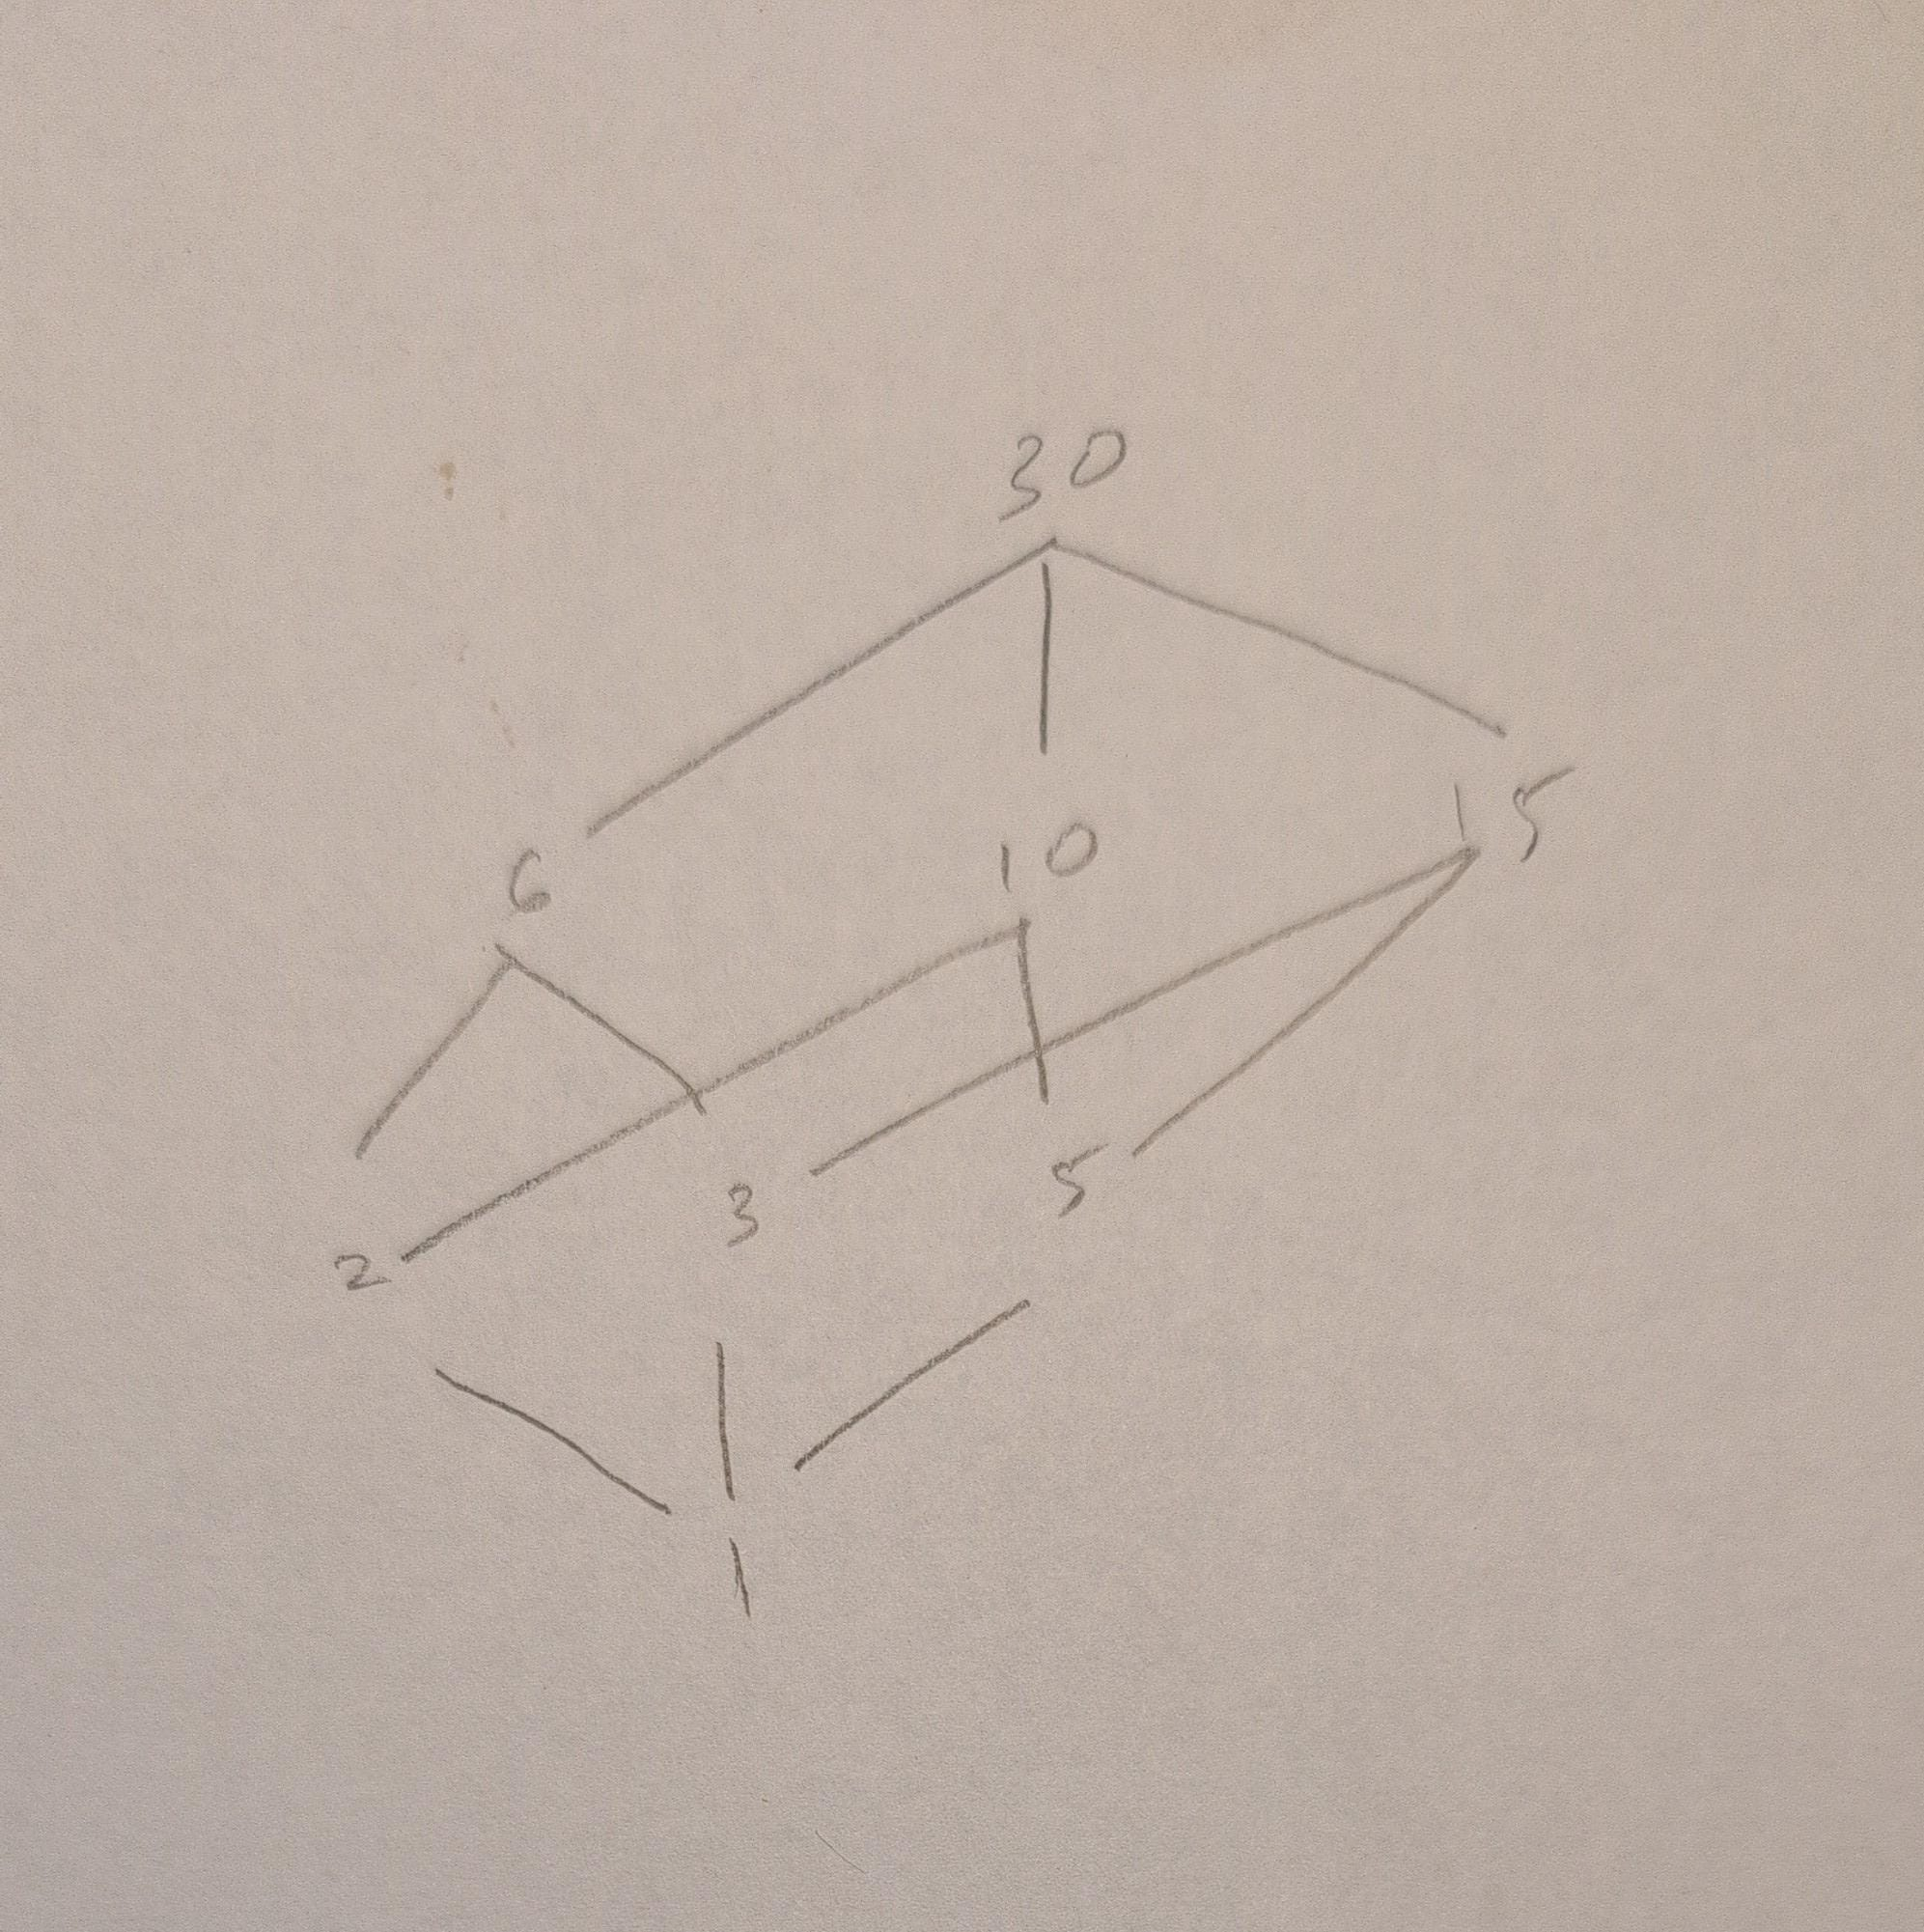
\includegraphics[scale=.2]{4}

\subsection*{Problem 5}
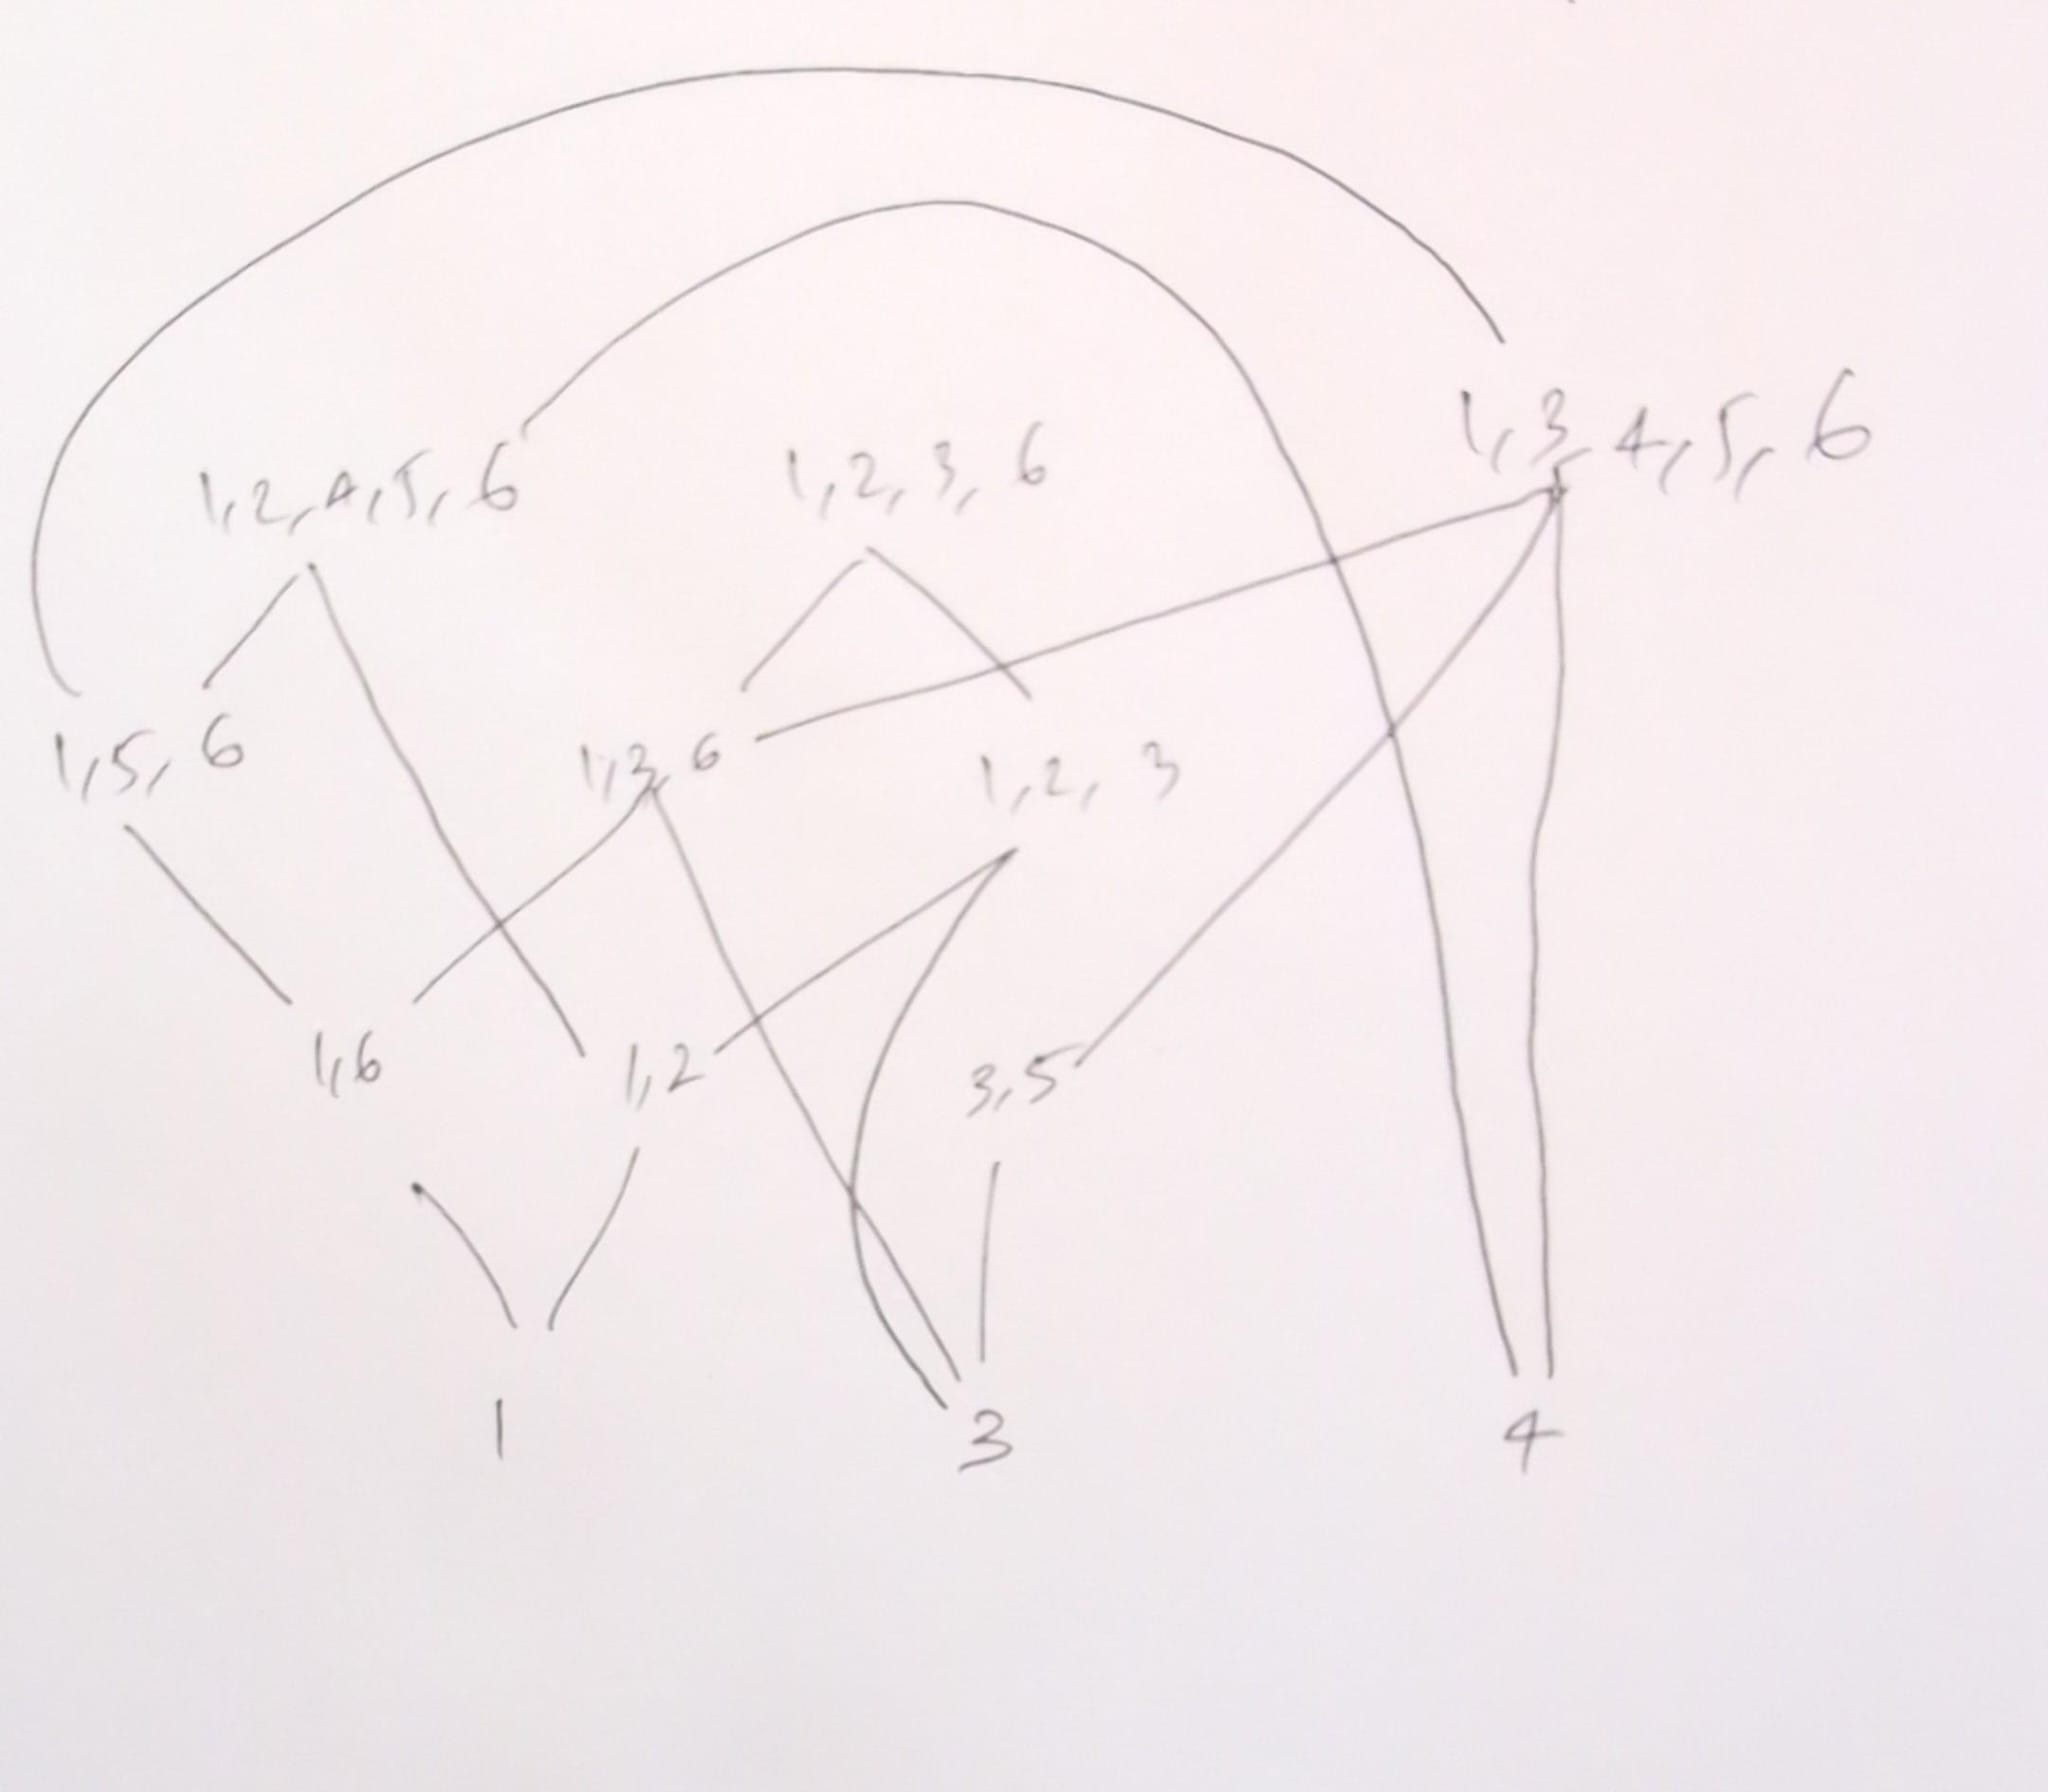
\includegraphics[scale=.2]{5}


\subsection*{Problem 6}
(1). 
$$ [\{3\}, \{2\}, \{3,7\},\{2,5\}, \{2,3,11\}, \{2,3,5,7\}, \{2,5,25\}] $$ 


(2). 
$$ [2, 3, 10, 66, 21, 50, 210] $$ 


(3). 
$$ [(1,2,1), (3,3,2), (4,1,5), (2,5,4), (6,4,5), (5,7,3), (7,6,7)] $$ 


\subsection*{Problem 7}
They would have the same height and width. This is because $P^{d}$ is the dual of $P$ and the longest chain in $P$ would be the longest chain in $P^{d}$ and similarly the longest antichain in $P$ would be the longest anti chain in  $P^{d}$. And because $Q$ is isomorphic to $P^{d}$ they share the longest chains and antichains. Hence $Q$ will have height 5 and width 3 as well.

\subsection*{Problem 8}
a. The maximal elements of $P$ are, 
$$ 15, 8, 11, 2, 17, 3 $$ 

b. The minimal elements are, 
$$ 16, 1, 5, 14 $$  

c. Maximal chain with two points are, 
$$ 16, 8 $$ 

d. $5, 6, 10$ is a chain with three points but is not maximal because it is a subset of the chain  $5,6,10,2$. And we know that the maximal chain is not a subset of any other chain.

e. $16, 1, 5, 14$ is a maximal antichain with 4 points.

\subsection*{Problem 9}
the $h$ anti-chains are, 
\begin{align*}
    h_1 &=12, 22, 23, 18, 16\\
    h_2 &=  3, 2, 21, 13, 11, 17\\
    h_3 &=  25, 4, 10\\
    h_4 &= 5, 24, 8\\
    h_5 &= 20\\
    h_6 &= 9, 19\\
    h_7 &= 6, 7\\
    h_8 &= 1, 26\\
    h_9 &= 14, 15
\end{align*}

So the height $h = 9$.
\subsection*{Problem 11}

We have $10$ different items and if we consider a poset where the order is defined by  inclusion our solution will be the largest antichain of the poset as they are the largest set which  are non comparable (they don't contain each other). So using Sperner's theorem we have, 
$$ width(2^{10}) = {10 \choose 5} $$ 
which is our solution.
\subsection*{Problem 13}
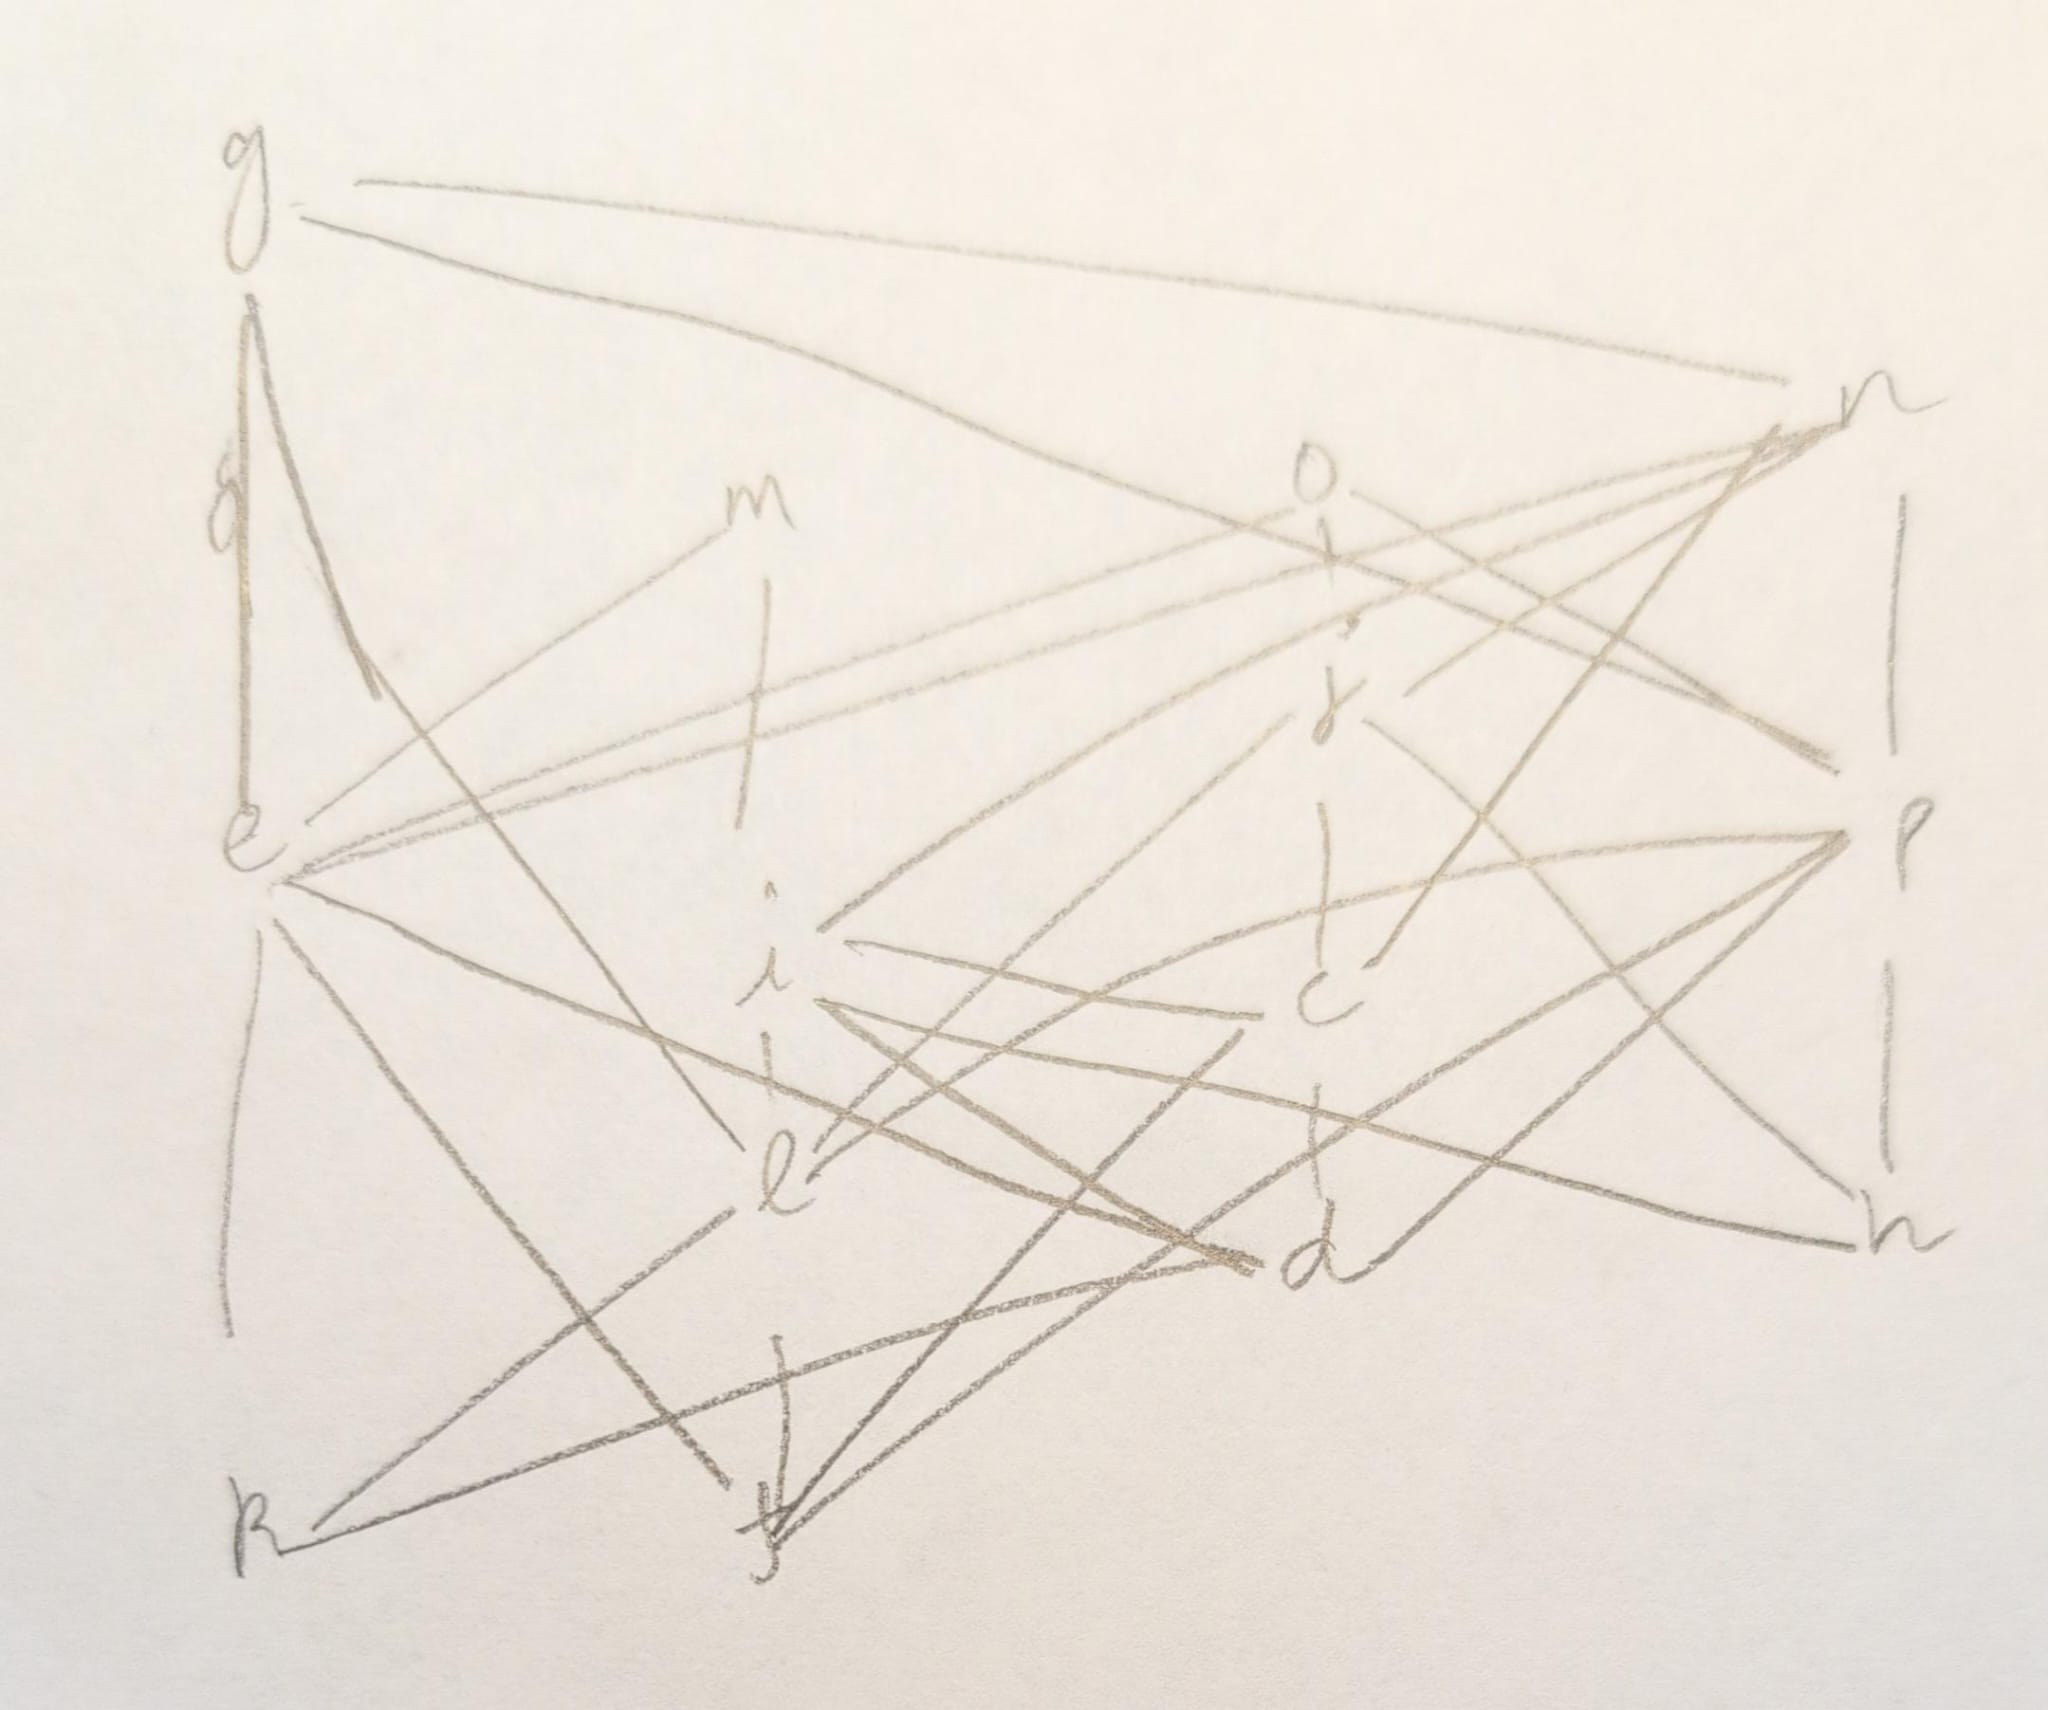
\includegraphics[scale=.2]{13}

\subsection*{Problem 14}

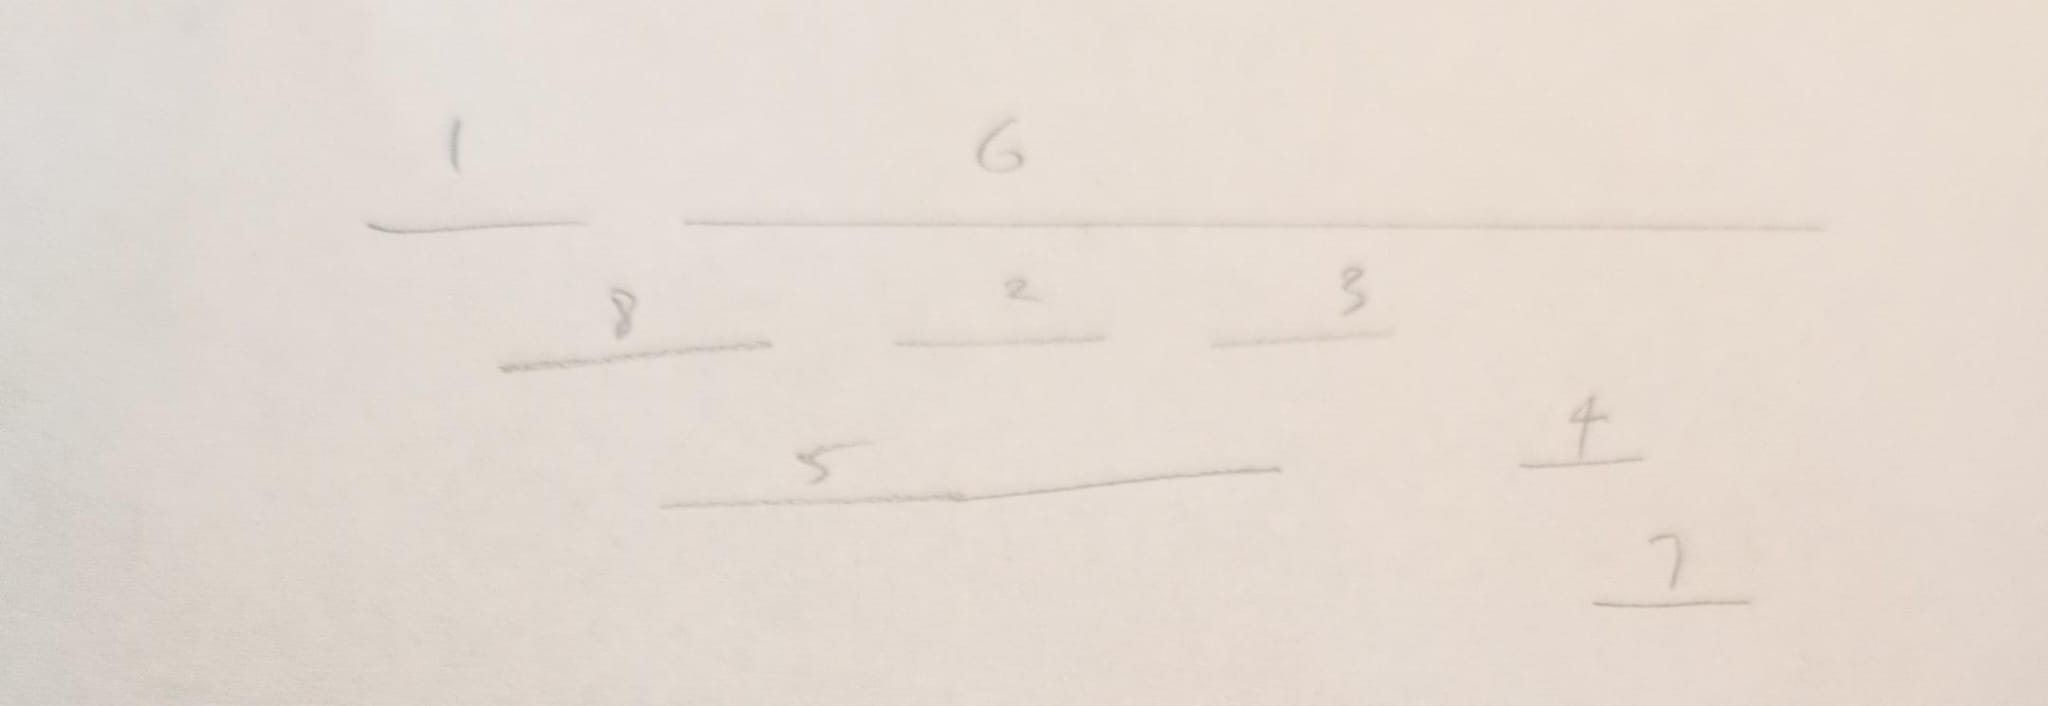
\includegraphics[scale=.20]{14}


\end{document}
